 \documentclass{article} %A4
\usepackage[a4paper,left=1.9cm, right=2.1cm,top = 1.2cm,bottom=2.3cm]{geometry}
\usepackage[utf8]{inputenc}%Umlaute
\usepackage[ngerman]{babel} %Texttrennung
\usepackage{graphicx}	%Grafiken
\usepackage{amssymb}
\usepackage{amsmath}
\usepackage{url}
\usepackage{listings}
\usepackage{color}
\usepackage{hyperref}
\usepackage{framed}
\usepackage{algpseudocode}
\usepackage{tikz}
\usepackage{enumitem}
\usepackage[xindy]{glossaries}
\makeglossaries
\usepackage[labelformat=empty]{caption}
\title{Zusammenfassung - Advanced Communications}
\author{
	Marc Meier, CD
}




\begin{document}
\maketitle
\begin{framed}Korrektheit und Vollständigkeit der Informationen sind nicht gewährleistet.
Macht euch eigene Notizen oder ergänzt/korrigiert meine Ausführungen!
\end{framed}
\setcounter{tocdepth}{1}
\tableofcontents
\newpage

\section{Grundlagen}

% 010, 020
\subsection{Grundprinzipien und Entwicklung des Internets}
Das Internet entwickelte sich ab den 1960er Jahren.
Es ging aus dem am Ende des Jahrzehnts entstandenen, vornehmlich militärisch und akademisch geprägten ARPA-Net hervor.
Heutzutage wird es international kommerziell, industriell und auch akademisch (Katzenbilder) genutzt.
Bei seiner Entstehung war vor allem eine dezentrale Struktur ohne zentrale Verwaltung von Interesse.
Grund hierfür war die Angst des amerikanischen Department of Defense, dass eine atomarer Angriff zentrale Kommunikationspunkte außer Kraft setzen könnte.
Die Kommunikation findet über hochgradig vernetzte Knoten mithilfe von Paketen statt.

Literatur: \cite{abbate2000inventing, baran1964distributed}
\subsection{Packet Switching}
Paketvermittelte Übertragung bedeutet die Abkehr von der leitungsbasierten Vermittlung.
Dabei werden längere Nachrichten in Datenpakete aufgeteilt und voneinander unabhängig versendet.
Dies ermöglicht eine faire Verteilung der Leistungskapazität und redundante Wege bei einem Ausfall von Knoten oder Verbindungen.
Im Gegenzug können konstante Bandbreiten nicht ohne Weiteres (Abschnitt \ref{sec:qos}) gewährleistet werden, ebenso ergeben sich unterschiedliche Laufzeiten von Paketen.

\subsection{Dezentrale Verwaltung des Internets}

\subsubsection{Prinzipien}

\begin{itemize}
\item Keine zentrale Verwaltung oder Behörde (trotz Einflussnahme)
\item Demokratisches Zusammenwirken der Beteiligten / Wahlen
\item Selbstorganisation
\item Standards dort, wo sie erforderlich sind
\item Dynamisch, offen für Neuigkeiten	
\end{itemize}

\subsubsection{Organisationen}

\begin{description}
\item [ICANN:] Vergibt IP-Adressen und betreibt die DNS-Rootserver.
\item[IETF:] Standardisierung von Protokollen in RFCs \cite{rfc3233}
\item[RIPE:] Administration und technische Koordination
\item[RIPE NCC:] Adressvergabe in Europa und Zentralasien, Verwaltung der WHOIS-Datenbank.
\item[DENIC eG:] Domain-Verwaltung für die Zone .de
\end{description}

\subsection{Standards}
Standards ermöglichen die Kooperation im Netzwerk, nur durch sie können Geräte verschiedener Hersteller miteinander kommunizieren.
Sie können textuell, mithilfe einer Referenzimplementierung oder anhand von Automaten (meist für zustandsbehaftete Protokolle) festgelegt werden.

\begin{description}
\item[Protokoll] Standardisierte Regeln (Vorschriften) und Vereinbarungen zu
Form, Ablauf, Steuerung und Sicherung (Fehler) der
Datenübertragung in und zwischen Rechnernetzen, zwischen
Einzel-Rechnern und zwischen Rechnern und
Peripheriegeräten.
\item[Standard] Ein Standard wird von den verschiedensten internationalen und
nationalen Organisationen sowie von großen Firmen erstellt.
Ein Standard wird als verbindliche oder unverbindliche
(empfohlene) Festlegungen schriftlich niedergelegt.
\end{description}

Ablauf einer Standardisierung bei RFCs:
\begin{enumerate}
	\item \textbf{Proposed Standard}: Vollständige, konsistente Spezifikation vorhanden
	\item \textbf{Draft Standard}: Mindestens 2 unabhängige, interoperable Implementierungen
	\item \textbf{Standard}: Operationell stabil
\end{enumerate}
\textbf{Weitere Status:} \emph{Experimental}, \emph{Informational} und \emph{Historic}.
\subsection{Netze, Autonome Systeme und Schichten}
Große Teile des Internet-Backbones werden von wenigen Firmen bereitgestellt (Tier-1).
Diese werden an einigen Knotenpunkten verbunden.
Wichtiger Knotenpunkt in Deutschland ist DE-CIX in Frankfurt/Main.
Man unterteilt folgende \textbf{Netzwerk-Schichten}:
\begin{description}
	\item[Tier 1]: Ein Netzwerk, das mit allen anderen Tier-1-Netzwerken verbunden ist; \emph{Internet-Backbone}; z.B. ATDN, GX, AT\&T...
	\item[Tier 2]: Netzwerk, das mit vielen Netzwerken verbunden ist, aber Transit \emph{einkauft}, um einige Bereiche des Internets zu erreichen; z.B. Deutsche Telekom
	\item[Tier 3]: Ein Netzwerk, das ausschließlich Transit \emph{einkauft}, um das
	Internet zu erreichen
\end{description}
\textbf{Autonome Systeme} sind Ansammlungen von IP-Netzen, die als Einheit verwaltet werden.
Innerhalb kommt ein einheitliches Routing-Protokoll zum Einsatz.
Autonome Systeme sind untereinander verbunden und
bilden das Internet.
\section{Protokolle}

\subsection{Zustandslose und zustandsbehaftete Protokolle}
Bei \textbf{zustandslosen Protokollen} wird jede Anfrage in einer eigenständigen Transaktion ausgeführt, es existieren keine Vorbedingungen oder Sitzungsinformationen (UDP, HTTP, TFTP).
\textbf{Zustandsbehaftete Protokolle} hingegen merken sich den aktuellen Zustand mithilfe einer Sitzung.
Nachfolgende Anfragen können auf die Sitzungsinformationen zugreifen.
Diese Zustandsübergänge können durch endliche Automaten dargestellt werden.
Beispiele sind FTP, TCP und SMTP.

\subsection{OSI-7-Schichten-Modell}

\begin{enumerate}
	\item Physical Layer / Bitübertragung
	\item Data Link Layer / Sicherungsschicht / Datenübertragungsschicht
	\item Network Layer / Vermittlungsschicht
	\item Transport Layer
	\item Session Layer / Sitzungsschicht
	\item Presentation Layer / Darstellungsschicht
	\item Application Layer / Anwendungsschicht
\end{enumerate}

Gute \textbf{Eselsbrücken} sind:
\begin{itemize}
	\item Alle deutschen Studenten trinken verschiedene Sorten Bier (deutsche Bezeichnungen, 7-1)
	\item An dem Samstag trug Verena 'nen String in Blau (deutsche Bezeichnungen, 7-1)
	\item Alle poppen Susis Tante nach der Party (deutsche Bezeichnungen, 7-1)
	\item Physiker, die nicht trinken sind potentielle Attentäter (deutsche/englische Bezeichnungen, 1-7)
	\item Alibaba präsentiert sich täglich nackt dem Personal
	\item  Please Do Not Throw Salami Pizza Away (englisch, 1-7)
\end{itemize}

Jede Schicht $n$ nutzt die darunterliegende Schicht $n-1$ um mit dem Kommunikationspartner zu kommunizieren.
Daten höherer Schichten werden in niederen Schichten umkapselt.
Die Bezeichnung der Pakete ist je nach Schicht unterschiedlich:
\begin{description}
	\item[Data Link Layer]: (Ethernet-)Frame
	\item[Network Layer]: Paket
	\item[Transport Layer]: Fragment
\end{description}

\subsection{Ethernet}
\label{subsec:ethernet}
Das Ethernet-Protokoll wirkt auf den Layern 1 + 2 und wird im Standard \textbf{IEEE 802.3} definiert.
Es kümmert sich um Elektrokrams (Physikalische Eigenschaften, Stecker,Stromversorung, Kabel etc.), Zugriffsverfahren auf das Medium, Adressierung (MAC), Protocol-Multiplexing, Flow Control (Logical Link Control) und Fehlererkennung (CRC).
Es ähnelt den Standards \textbf{802.11} (WLAN), \textbf{802.15.1} (Bluetooth) und \textbf{802.16} (WiMAX).

Ein \textbf{Ethernet-Frame} hat eine Größe von 64 - 1518 Byte.
Davon ausgenommen sind die Präambel und der SFD.
Wird das VLAN-Tag genutzt, sind 1522 Byte möglich.
Das \textbf{Ethernet-Paket} (Offensichtlich Präambel + SFD + Ethernet-Frame) umfasst folgende Felder:

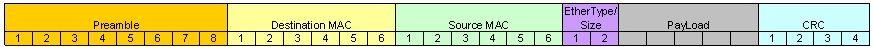
\includegraphics[width=16cm]{img/EthernetFrame.jpg}

\begin{description}
	\item[Präambel]: Zum Synchronisieren von Sender und Empfänger, \emph{Einschwingphase} (8 Byte)
	\item[SFD]: Festgelegte Sequenz 10101011 (1 Byte)
	\item[Ziel-Mac-Adresse]: Adresse des Empfängers (8 Byte)
	\item[Quell-Mac-Adresse]: Adresse des Senders (8 Byte)
	\item[VLAN-Tag]: Nach IEEE 802.1q, optional (4 Byte)
	\item[Typ-Feld]: Identifiziert die Art des nachfolgenden Inhalts, z.B. IP, ARP, etc...
	\item[Nutzlast]
	\item[PAD-Füllfeld]: Wird optional benötigt, um die Mindestlänge von 64 Byte einzuhalten \footnote{Rausfinden, warum mindestens 64 Byte nötig. Vermutung: Kollisionserkennung}
	\item[CRC-Prüfsumme]: Zur Fehlererkennung (4 Byte)
\end{description}

\subsubsection{CSMA/CD}

CSMA/CD regelt den Zugriff auf ein von mehreren Teilnehmern genutztes Medium (Kabel).
Dazu prüft der sendene Host, ob das Medium frei ist, bevor er sendet.
Beim Übertragen von Daten können Kollisionen erkannt werden.
Der Sendevorgang wird dann nach einer zufälligen Zeit wiederholt.
Aufgrund der verbreiteten Nutzung von Switches sind echte geteilte Medien inzwischen eher die Ausnahme.

$\Rightarrow$ Jeder Port am Switch bildet eine eigene \emph{Kollisionsdomäne}.
Die Bustopologie mit Koaxialkabeln (aber auch mit Hubs) wird nicht mehr genutzt.

\subsubsection{Duplex / Half Duplex}

Beim \textbf{Full Duplex} sind beide Seiten in der Lage, gleichzeitig zu Senden und zu Empfangen.
Im Falle von \textbf{Half Duplex} ist dies nur wechselseitig möglich (vgl Walkie Talkie).
Es sind verschiedene Realisierungen einer geteilten Nutzung eines Mediums möglich:

\begin{description}
	\item [Zeitduplex (TDD)]: Übertragung in verschiedenen Zeitschlitzen
	\item [Frequenzduplex (FDD)]: Übertragung auf verschiedenen Frequenzen
	\item [Codeduplex]: (nicht im Skript)
\end{description}

\subsection{Switching}

\textbf{Switches} sind Geräte auf dem OSI-Layer 2.
Sie empfangen Ethernet-Frames und leiten sie anhand ihrer Empfänger-MAC-Adresse weiter.
Im Gegensatz zum Hub wird dabei nur über den Port ausgegeben, hinter dem sich der Empfänger befindet.
Die Ausnahme ist hierbei, wenn der Port des Empfängers nicht bekannt ist.
Anhand der empfangenen Frames lernt ein Switch, wo sich Geräte befinden.

\subsubsection{Realisierungsmöglichkeiten}

%TODO Switches - Realisierungsmöglichkeiten

\subsubsection{Cut-Through und Store-and-Forward}

Beim \textbf{Cut-Through} (auch \emph{On The Fly Forwarding}) werden Pakete sofort nach Empfang der Empfängeradresse auf dem entsprechenden Port weitergeleitet, sofern dieser Frei ist.
Diese Methode ist sehr schnell (Verzögerung ca. 40$\mu$s), leitet jedoch gegebenenfalls auch fehlerhafte Frames weiter, da CRC umgangen wird.

\textbf{Store-and-Forward} hingegen empfängt zuerst den gesamten Frame, prüft diesen und leitet ihn anschließend weiter.
Offensichtlich werden keine fehlerhaften Pakete mehr in benachbarte Segmente weitergeleitet, dies wird jedoch durch erhöhte Latenz erkauft.

In der Praxis arbeiten Switches häufig im Cut-Through-Modus und schalten bei erhöhter Fehlerrate in den Store-and-Forward-Modus.

\subsubsection{VLAN}

Ermöglicht die Aufteilung von Switches in mehrere virtuelle LANs.
Den Ports werden dabei einzelne VLANs zugeordnet.
Auf diese Weise kann Hardware eingespart werden.
Realisiert wird dies mit einem 4 Byte langen Feld im Ethernet-Frame:
\begin{itemize}
	\item 2 Bytes \textbf{TPID} - Tag Protocol Identifier – Fester Wert 0x8100. Frame
	trägt die 802.1Q/802.1p-Tag-Information
	\item 3 Bit \textbf{Priorität} (user\_priority) – Benutzer-Prioritätsinformationen
	\item 1 Bit \textbf{CFI} - Canonical Format Indicator – Gilt für alle vorhandenen
MAC-Adressinformationen im MAC-Datenpaket des Frames. Wert 0
das Format ist kanonisch (am wenigsten signifikante Bit zuerst); Wert
1 Format nicht-kanonisch. Benutzung im Token Ring/Source-Routed-
FDDI-Media-Zugang, um die Bit-Order der Adressinformationen des
verkapselten Frames festzulegen
	\item 12 Bit \textbf{VID} - VLAN Identifier – Identifizierung des VLANs zu dem der
Frame gehört
\end{itemize}

\subsubsection{Trunking / Link Aggregation}
Ermöglicht die Zusammenfassung mehrerer Ports zur Erhöhung des Datensatzes.

\subsection{Asynchronous Transfer Mode}

%TODO ATM

\subsection{Internet Protocol}
\label{subsec:ip}
Beim Internet Protocol handelt es sich um ein Layer-3-Protkoll, weches auf die Layer-2-Protokolle Ethernet, ATM und FDDI aufsetzen kann.
Es verwendet globale, logische Adressen.
Aufgrund der Erschöpfung des IPv4-Adressraumes\footnote{Weitere Maßnahmen, dem entgegenzuwirken sind etwa: NAT, CIDR, DHCP, Private Adressräume} (32 Bit) wird nach und nach IPv6 eingeführt (128 Bit)

\subsubsection{IPv4}
Wurde im RFC 791\cite{rfc791} definiert.
Der Header eines IPv4 Paketes ist insgesamt 20 Byte lang.
Davon sind insbesondere die folgenden von Interesse:

\begin{description}
	\item [Version]: In diesem Fall \emph{4}, bei IPv6 offensichtlich \emph{6} (4 Bit)
	\item [Header Length]: Gesamtlänge des Headers kann 20 Byte überschreiben, wenn zusätzliche Optionen gesetzt werden. Angabe in 32-Bit langen Blöcken (4 Bit)
	\item [Total Length]: Gesamtgröße des Pakets. Nach RFC muss jeder Host in der Lage sein, mindestens Pakete mit einer Länge von 576 Bytes zu verarbeiten. (16 Bit)
	\item [Type of Service]: Type of Service nach RFC791(ursprünglich für Quality-of-	Service-Anwendungen gedacht)
	
	\begin{itemize}
		\item bits 0-2: precedence
		\item bit 3: 0 = Normal Delay, 1 = Low Delay
		\item bit 4: 0 = Normal Throughput, 1 = High Throughput
		\item bit 5: 0 = Normal Reliability, 1 = High Reliability
		\item bits 6-7: Reserved for future use
	\end{itemize}
	Heute anders verwendet zur Servicebeschreibung durch Dienstklassen (DiffServ, 8 Bit)
	\item [Identification]: Falls ein Paket fragmentiert wird, haben alle Fragmente die	selbe Identification.
	\item [Flags]: Reserved\cite{rfc3514}, Don't Fragment, More Fragments (3 Bit)
	\item [Fragment Offset]: Kann ein Paket nicht auf einmal übertragen werden (z.B. bei
	kleinerer Maximum Transfer Unit, MTU), wird es fragmentiert.
	FO gibt an, ab welcher Stelle (gemessen in Blöcken von 8 Byte)
	dieses Paket die Daten enthält (MF Flag ist gesetzt) (13 Bit)
	\item[TTL]: Anzahl der Hops, bis Paket verworfen wird
	\item [Options]: Beispielsweise für Source Routing (Route ist im Paket vorgegeben); Sehr selten verwendet, häufig blockiert oder ignoriert
\end{description}

\begin{center}
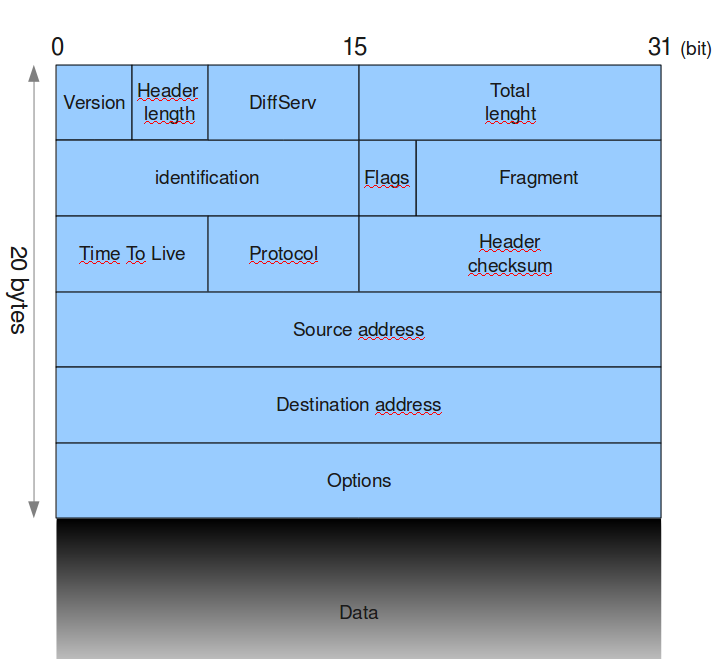
\includegraphics[width=8cm]{img/IP_packet}
\end{center}

Nutzung von Adressklassen\footnote{Class A 1.x.y.z-126.x.y.z; Class B 128.0.y.z-191.255.y.z; Class C 192.0.0.z-223.255.255.z} aufgrund der Verknappung der Adressen durch CIDR\cite{rfc1519} abgelöst.
Dies ermöglichte Super- und Subnetting.
Adressangabe bei CIDR im Format a.b.c.d/x, wobei x angibt, wie viele Bits zum Netz-Anteil der Adresse gehören.
Subnetze dienen zur Aufspaltung von Netzen in Teile, um diese besser handhaben zu können (Broadcast-Domains, Logische Strukturierung, Dezentrale Verwaltbarkeit)
\subsubsection{IPv6}

Die auffälligste Änderung von IPv4 zu IPv6 ist die vergrößerte Adressgröße (128 Bit).
Damit ergeben sich $3,4 \cdot 10^{38}$ Adressen.
IP - Adressen werden im Hexadezimalsystem zu je acht Word-Gruppen á 2 Bytes dargestellt.
Verkürzte Darstellung möglich durch Verzicht auf „Nullen“ in einer Gruppe (einmal je Adresse).
Es existieren IPv4-kompatible Adressen und die CIDR-Darstellung für Subnetze bleibt erhalten.
Weiterhin wurde die Anzahl der Felder im Header reduziert und (optionale) Erweiterungsheader hinzugefügt.
Wichtige Felder sind:

\begin{description}
	\item [Traffic Class]: \begin{itemize}
		\item 0 uncharakterisierter Verkehr
		\item 1 „Füllmaterial", z.B. Newsgroups
		\item 2 zeitunkritischer Verkehr, z.B. EMail
		\item 3 reserviert
		\item 4 Mengendaten, z.B. FTP, NFS
		\item 5 reserviert
		\item 6 Interaktive Anwendungen, z.B. telnet
		\item 7 Steuerung, z.B. SNMP
	\end{itemize}
	\item [Flow Label]: Anwendung kann Datenstrom mit einem Flow-Label versehen, z. B. bei Streaming-Anwendungen.
	Flow nicht notwendigerweise an Verbindung gebunden (logisch, da IP nicht verbindungsorientiert arbeitet).
	Empfänger kann Datenstrom am Flow Label erkennen. \cite{rfc3697, rfc6437}
	\item[Next Header]: Gibt an, dass ein weiterer Header folgt.
	In IPv6 sind viele Felder weggefallen.
	Next Header ermöglicht das anfügen eines weiteren Headers.
	RFC 2460\cite{rfc2460} bietet beispielsweise:
	\begin{itemize}
		\item Hop – by – Hop Options Header
		\item Routing Header
		\item Fragmentation Header
		\item Authentication Header
		\item Encapsulated Security Payload (ESP) Header
		\item Destination – Option – Header
	\end{itemize}
	 
\end{description}

\begin{center}
	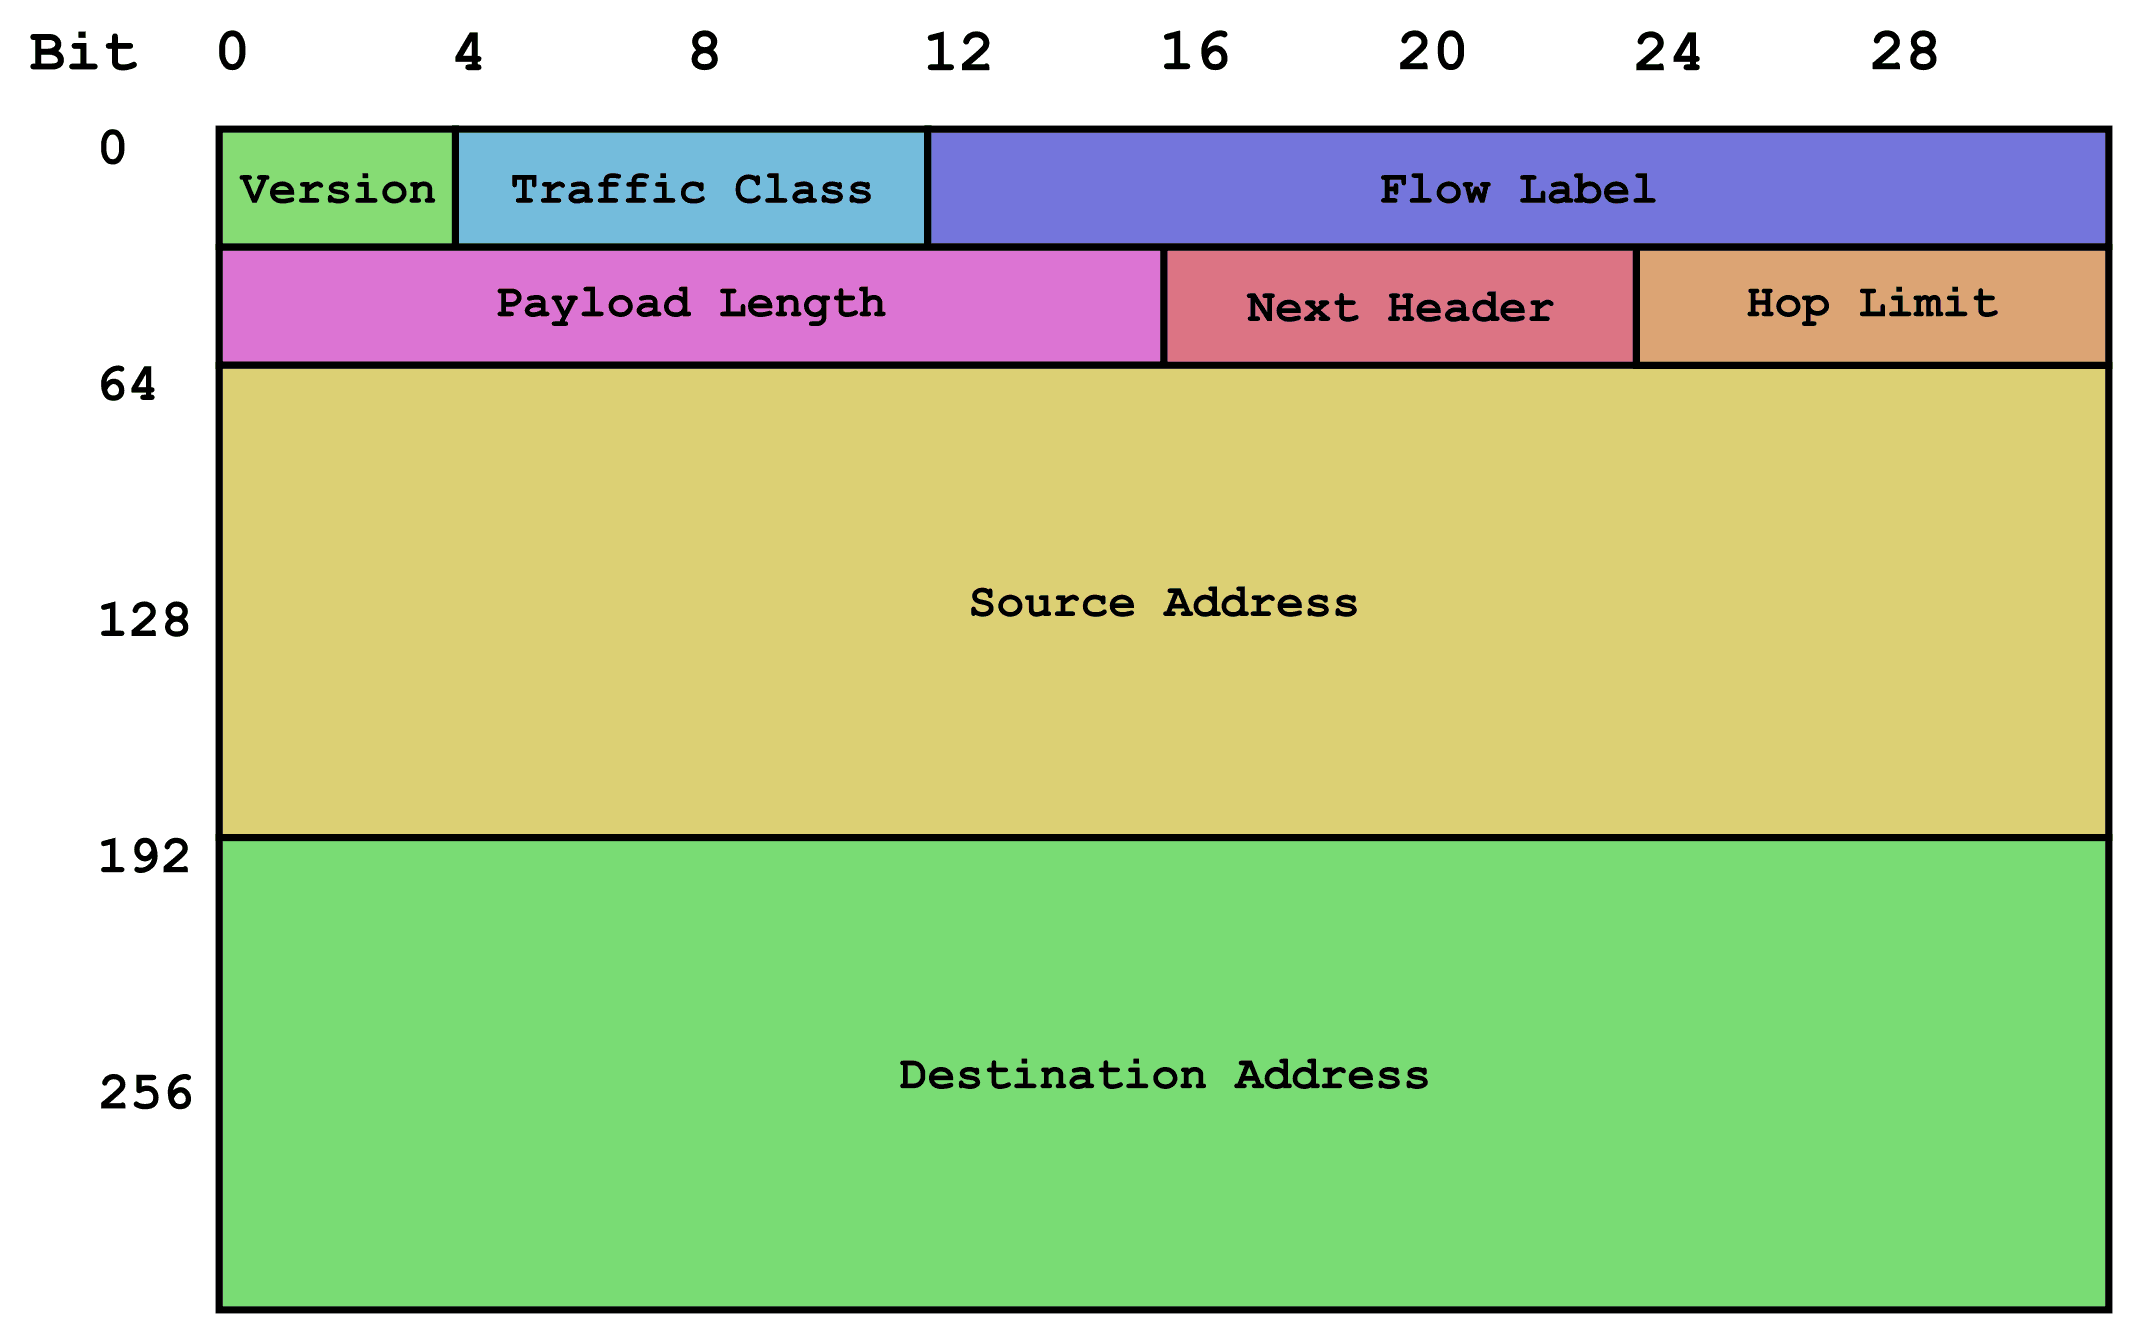
\includegraphics[width=10cm]{img/IPv6_header}
\end{center}

\subsection{User Datagram Protocol}

Bei UDP handelt es sich um ein Layer-4-Protokoll.\cite{rfc768}
Es dient zur Übermittlung kurzer Nachrichten an andere Systeme und garantiert weder Zuverlässigkeit noch Einhaltung der Reihenfolge der Pakete beim Empfänger.
Die Adressierung geschieht über Ports (16 Bit).
Der Header enthält 4 Felder (je 16 Bit): Quellport, Zielport, Datagram-Länge und eine Checksumme.

\subsection{Transmission Control Protocol}

TCP ist ebenfalls ein Layer-4-Protokoll.\cite{rfc793}
Es garantiert eine Ankunft der Pakete in korrekter Reihenfolge.
Clienten sehen die Verbindung als bidirektionalen Datenstrom, tatsächlich findet die Kommunikation über Pakete statt.

\subsubsection{Paketstruktur}

Der Header des TCP-Fragments ist 20 Byte groß.
Wichtige Felder sind:
\begin{description}
	\item [Sequence Number / Acknowledgement Number]: Zerlegung des Datenstroms in nummerierte Blöcke.
	Größe der Blöcke ist variabel (Nagle Algorithmus).
	Verwerfen von Segmenten mit fehlerhafter Prüfsumme.
	Bestätigung empfangener Segmente.
	Nicht unbedingt für jedes Segment einzeln (Windowing).
	Erneuter Transport unbestätigter Segmente.
	Zusammensetzung des Datenstroms auf Empfängerseite
	
	\item [Flags]: dienen unter anderem zur Steuerung des Verbindungsauf- und –abbaus.
	\begin{description}
		\item [URG] - Urgent Flag (Urgent Pointer enthält
			Sequenznummer, die bevorzugt übertragen werden soll)
		\item [ACK] – Acknowledgement
		\item [PSH] – Push (Paket wird sofort an Anwendung weitergeleitet, ohne Zwischenpuffer)
		\item [RST] – Reset (Unterbrechung der Verbindung)
		\item [SYN] – Synchronized (Aufbau der Verbindung)
		\item [FIN] – Finish (Beenden der Verbindung)
	\end{description}
	\item [Window Size]: Anzahl der Daten, die gesendet werden können bis ein Acknowledgement gesendet werden muss (in Bytes oder mit speziellem Option Header nach RFC1323 \cite{rfc1323} auch bis zu 1GB,	dann Linksverschiebung um bis zu 14 Bits, $2^{14} \cdot 64k = 1G$).
\end{description}

\subsubsection{Zustände}

Zum Aufbau einer Verbindung wird der \textbf{3-Way-Handshake} durchgeführt: $\rightarrow$ SYN | $\leftarrow$ SYN + ACK | $rightarrow$ ACK.
Ein Timeout findet typischerweise nach 75 Sekunden statt.

Zum Abbau der Verbindung genügt das Senden und Quittieren eines FIN.

\section{Adressierung}

% 030
\subsection{MAC-Adressen}

\begin{itemize}
	\item Layer-2-Adressen für Ethernet
	\item 6 Byte / 48 Bit groß
	\item \emph{Eigentlich} weltweit eindeutig
	\item \emph{Eigentlich} in Hardware gegossen, trotzdem fälschbar
	\item Darstellung: Hexadezimal, Bits getrennt durch \[.:-\]
	\item Bit 3 bis Bit 24 an Hersteller gebunden (z.B. 00-60-2F-xx-xx-xx für Cisco)
	\item Broadcast: FF-FF-FF-FF-FF-FF 
\end{itemize}

\subsection{VPI und VCI bei ATM}

%TODO VIP und VPI bei ATM

\subsection{IP-Adressen}

Siehe Abschnitt \ref{subsec:ip}.

\subsection{Ports}

Für die Layer-4-Protokolle UDP und TCP werden 16-Bit-Adressen verwendet.
Diese werden als Ports bezeichnet.
Ports 0-1023 sind dabei standardisiert.
Wichtige Portnummern sind beispielsweise:
\begin{center}
\begin{tabular}{|c|c|c|c|}
	\hline Port & TCP & UDP & Beschreibung \\ 
	\hline 20 & Ja & Nein & FTP - Datenübertragung \\ 
	\hline 21 & Ja & Nein & FTP - Kontrolle \\ 
	\hline 22 & Ja & (Ja) & SSH \\ 
	\hline 23 & Ja & Nein & Telnet \\ 
	\hline 25 & Ja & Nein & SMTP \\ 
	\hline 53 & Ja & Ja & DNS \\ 
	\hline 80 & Ja & Nein & HTTP \\ 
	\hline 110 & Ja & Nein & POP3 \\ 
	\hline 123 & Nein & Ja & NTP \\ 
	\hline 443 & Ja & Nein & HTTPS \\ 
	\hline 
\end{tabular} 
\end{center}
\subsection{URIs, URNs und URLs}
\begin{description}
\item [Uniform Resource Identifier]: String; Benennt oder identifiziert eine Ressource z.B.  \textbackslash\textbackslash139.30.3.23\textbackslash iukp\textbackslash beispiel.txt
\item [Uniform Resource Name]: Sonderform der URI, die eine Ressource in einem bestimmten
Namespace benennt | urn:ip-addr:139.30.3.23
\item [Uniform Resource Locator]: Sonderform der URI, die zusätzlich das Protokoll angibt, über das die Ressource erreichbar ist z.B. http://139.30.3.23/beispiel.txt
\end{description}
\subsection{*cast} 
\begin{description}
	\item[Unicast]: Einer sendet an einen, wie beispielsweise in einer TCP-Verbindung für HTTP. Adressierung durch Angabe des Empfängers.
	\item[Broadcast]: Einer sendet an alle, wie beispielsweise in ARP oder DHCP. Hierzu werden spezielle Adressen (MAC: FF-FF-FF-FF-FF-FF; IP: höchste Adresse im Subnetz) verwendet.
	\item[Multicast]: Einer sendet an viele Mitglieder einer Gruppe. Siehe Abschnitt \ref{sec:muliticast}.
	\item[Concast]: Viele senden an einen, Nachrichten werden so früh wie möglich zusammengefasst. Verhindert Implosion, Überlastung des Empfängers. Beispielswiese sinnvoll, wenn Fehlermeldungen zusammengefasst werden können. Keine direkte Unterstützung in IP
\end{description}

%TODO Foliensatz enthält noch ICMPv6 Neighbor Discovery Protocol, Domainverwaltung und Domain Registry
\section{ARP, RARP}

% Ende 030, 040

ARP sendet Layer-3-Adressen in Layer-2-Adressen um.
Es beschränkt sich nicht auf das erfragen von MAC-Adressen zu IP-Adressen, sondern ermöglicht beispielsweise auch ATM ARP, IP over FDDI und IP over Token Ring.
\begin{itemize}
	\item Erfragt für gegebene IP-Adresse eine MAC-Adresse.
	\item Host erzeugt Broadcast.
	\item Der angefragte Host darf darauf antworten (Unicast).
	\item Nachdem der Sender der Broadcast-Nachricht die Antwort erhalten hat, kann er die IP-Adresse der Ethernet-Adresse zuordnen.
	\item Diese Ethernet-Adresse wird dann für alle folgenden Pakete an diese Internet-Adresse verwendet, solange bis die Cache-Zeit abgelaufen ist.
	\item RFC 826 \cite{rfc826}
\end{itemize}

\subsection{Einsatzfälle}

\begin{enumerate}
	\item Zwei Hosts möchten im selben Netzwerk (ausschließlich Layer 2) miteinander kommunizieren und kennen nur die Layer-3-Adresse (z.B. IP-Adresse) des Empfängers.
	\item Ein Host benötigt die Layer-2-Adresse des Gateways, um andere Netze zu erreichen (Sonderfall des zuvor genannten)
	\item Zwei Gateways wollen kommunizieren.
\end{enumerate}

\subsection{Paketstruktur}
Wichtige Felder eines ARP-Requests sind:
\begin{description}
	\item[Hardware type]: Kennzeichen für die verwendeten Hardware-Adressen (1 für Ethernet, 2 Byte)
	\item[Protocol type]: Kennzeichen für die verwendeten Protokoll-Adressen (L3) (0x0800 für IPv4, 2 Byte).
	\item[Hardware length]: Länge der Hardware-Adresse in Bytes (6 für Ethernet, 1 Byte)
	\item[Protocol Length]: Länge der Protokoll-Adressen (L3) (4 für IPv4, 1 Byte)
	\item[Operation]: Unterscheidung von 1 Request und 2 Reply, da für beides gleiche Pakete verwendet werden (2 Byte, warum zur Hölle reserviert man für 2 Werte 2 Byte?)
\end{description}

Es folgen Sender hardware address, Sender protocol address, Target hardware address und Target protocol address

\subsection{ARP-Caching}

Um nicht für jedes IP-Paket einen neuen ARP Request zu stellen, werden die Ergebnisse zwischengespeichert.
Typischerweise 10 Minuten lang.
Kommt es während der Cache-Zeit zu einem Fehler (Host nicht erreichbar), wird erneut ein ARP-Request ausgeführt.

\subsection{ARP-Announcements}

Der anfragende Host sendet bekanntlich einen Broadcast, alle Host im gleichen Netz können folglich diese Information ebenfalls verwenden, und auf diese Weise eigene Anfragen sparen.
Anwendungen:
\begin{itemize}
\item Unterbrechungslose Übernahme einer Protokoll-Adresse (z.B. IP-Adresse) in hochverfügbaren Systemen.
\item Der anfragende Host kann auf diese Weise feststellen, ob eine Protokoll-Adresse bereits vergeben ist (Gratuitous ARP). Dieser Mechanismus wird bei IP-Autoconf verwendet.
\end{itemize}

IP-Autoconf \cite{rfc3927} ist eine einfache Möglichkeit zur Adresskonfiguration ohne Server (DHCP, RARP).

\begin{itemize}
	\item Host wählt zufällig eine Adresse.
	\item Überprüft mittels Gratuitous ARP, ob diese Adresse bereits vergeben ist.
	\item Falls ja, andere Adresse zufällig wählen und erneut überprüfen.
	\item Falls nein, Adresse benutzen und andere ARP Requests für diese Adresse beantworten.
\end{itemize}

\subsection{ARP-Spoofing}

Da ARP nicht kryptografisch abgesichert ist, kann jeder Host auf ARP Requests antworten oder ARP Announcements erzeugen.
Ziel ist das Umleiten von Datenpaketen.
Es gibt Programme, die Änderungen der Hardware-Adressen erkennen (z.B. arpwatch).
Der Administrator muss dann die Ursache überprüfen

\subsection{Proxy ARP}

Wird von speziellen Routing-Protokollen verwendet.
Jeder Nachbar (One-Hop-Neighbor), der auf der Route zum Ziel liegt, beantwortet einen eintreffenden ARP-Request mit seiner Hardware-Adresse.
Pakete werden so von Host zu Host weitergeleitet

\subsection{Reverse RP}

Erfragt eine IP-Adresse bei bekannter MAC-Adresse und ist nicht unbedingt für die Funktionsfähigkeit von IP über Ethernet notwendig.
RARP wird in RFC 903 \cite{rfc903} standardisiert.
Haupteinsatzzweck ist die automatische Konfiguration der Protokoll-Adresse.
Dabei sendet der Host einen RARP-Request mit der eigenen Hardware-Adresse (z.B. MAC).
Ein RARP-Server beantwortet diesen Request und liefert die hinterlegte Protokoll-Adresse (z.B.IP).
Da RARP Link-Local-Broadcasts verwendet, ist ein RARP-Server pro Netz notwendig.
Benutzt gleiche Paketstruktur wie ARP, lediglich anderen EtherType\footnote{Feld im Ethernet-Header, siehe Abschnitt \ref{subsec:ethernet}} (0x8035)

\section{DNS und WHOIS}

% 050
%TODO Ordnung in die Informationen bringen. Folien haben keinen guten roten Faden
Die Aufgabe des Domain Name Systems ist die Übersetzung von (Layer-4) IP-Adressen in, für den menschlichen Gebrauch besser verwendbare Namen.
Der Name wird dabei aus hierarchischen Domains, getrennt durch Punkte (.) zusammengesetzt.
Direkt unter der Wurzel steht hierbei die sogenannte Top-Level-Domain.
Bei Top-Level-Domains wird zwischen \textbf{länderspezifischen} (ccTLD) und \textbf{generischen} (gTLD) Domains unterschieden.
Während erstere, bestehend aus zwei Buchstaben, durch lokal verantwortliche Institutionen\footnote{Network Information Centers z.B. DENIC für .de} verwaltet werden, werden gTLD durch die ICANN oder beauftragte Institutionen vergeben.
%TODO 050_DNS.pdf hat hier noch so eine komische Seite 61
Bei der Vergabe gilt das \emph{first come, first serve}-Prinzip.
Für die Namensbildung gelten gewisse Regelungen, z.B. Ziffern 0-9, Bindestriche, Buchstaben, sowie einige ausgewählte lokale Buchstaben.
Letztere müssen ASCII-kodierbar sein (ACE)\cite{rfc3490}.
Jede (Teil-) Domain ist maximal 63 Zeichen lang, insgesamt ist der vollständige Pfad jedoch 255 Zeichen lang.
Folgende Daten sind bei der Domainanmeldung von Interesse:

\begin{description}
	\item[Domaininhaber](Holder): Person, der die Domain \emph{gehört}
	\item[Administrativer Ansprechpartner]: Vom Inhaber Bevollmächtiger, darf alle Entscheidungen treffen (Admin-C)
	\item[Technischer Ansprechpartner, Zonenverwalter]: Typischerweise Kontaktadresse der Firma, die die Domain betreibt (Tech-C, Zone-C)
	\item [Technische Daten]: z.B. Nameserver
\end{description}

Hoster tragen oft nicht den Inhaber selbst als Admin-C, sondern sich selbst ein.
Außerdem stellen sie in der Regel den Nameserver zur Verfügung.
Die Registrierung einer Domain gilt immer für einen bestimmten Zeitraum.
Ein Wechsel erfordert eine Freigabe beim alten Provider durch Inhaber oder Admin-C.

\subsection{Weiteres Bla zu DNS}

Beim Domain Name System handelt es sich um ein \textbf{sehr großes}, \textbf{hierarchisch strukturiertes}, \textbf{verteiltes}, \textbf{repliziertes} und \textbf{lokal verwaltetes System} \cite{rfc1034,rfc1035}.
Aus dem hierarchischen Benennungsschema resultiert das verteilte Datenbanksystem des DNS.
Jede Domain bestimmt selbst, wie die unter ihr liegenden Domains zugewiesen werden, hat dementsprechend eigene Verantwortlichkeiten.
Ist ein Namensserver für eine solche Zone verantwortlich, kann er Anfragen autoritativ beantworten(Autoritäskonzept).
Andernfalls wird die Anfrage aus dem Cache beantwortet oder an einen anderen Nameserver delegiert (Delegationskonzept).
Das kann der Nameserver einer Subdomain oder (default) ein Root Name server sein.

\subsection{Servertypen}

\begin{description}
\item[Primary Server]: Ist Hauptserver einer Domain und autorisiert, Anfragen zu seiner Domain verbindlich zu
beantworten.
Er verfügt über alle Daten dieser Domain, welche in Zonen-Dateien abgelegt sind, die der Verwalter des
Servers erstellt
\item[Secondary Server]: Ist ebenfalls autorisiert, verbindliche Antworten zu seiner
Domain zu liefern, lädt die Domain-Datenbank von einem Primary Server und aktualisiert sie bei Bedarf
\item[Caching-only Server]: Verfügt über keine eigenen Domain-Informationen.
Fragt bei dem für die Domain zuständigen Primary oder Secondary Server nach und speichert die Antwort zwischen
Ist zur Beantwortung von Anfragen zu einer Domain „nicht autorisiert“ (kann die Genauigkeit und Aktualität nicht gewährleisten)
\item[Slave	Server]: Reicht alle Anfragen, die er selbst nicht aus seinem eigenen Cache beantworten kann, an eine zuvor festgelegte Liste von anderen Servern (Forwarders) weiter.
Forwarders fragen ihrerseits den zuständigen Server und speichern Ergebnis zwischen (Caching)
\end{description}



\section{Migration von IPv4 nach IPv6}

% 060

\section{Timeouts, ACK, Bestätigungen}

% 070

\section{Routingkonzepte}

% 080, 090, 095, 100, 110, 120, 130

\section{Quality of Service}
\label{sec:qos}
% 140

\section{Multicast}
\label{sec:muliticast}
% 150, 180

\section{Zeitsynchronisation}

% 160, 190

\section{Internet Control Message Protocol}

% 170

\section{Voice over IP}

% 200, 210

\section{World Wide Web und HTTP}

% 220, 230

\section{Peer-to-Peer}

% 240, 250

\section{E-Mail}

% 260

\section{Autokonfiguration}

% 280, 290

\section{Dateien und Drucken}

% 300, 310

\section{Telnet, SSH und rlogin}

% 320

\section{Extensible Messaging and Presence Protocol (XMPP)}

% 330

\section{LDAP}

% 340

\section{Authentication Protocols}

% 350

\section{Simple Network Management Protocol}

% 360 

\section{Mac-Sublayer}

% 365

\section{Mobile Netzwerke}

% 370, 380, 390, 400

\section{HTTP2 und SCTP}

% 410

%TODO \nocite{*} soll alle Literaturverweise anzeigen, auch wenn diese im Text nicht auftauchen. Funktioniert bisher allerdings nicht so

%TODO Eventuell Literaturverzeichnis über zwei Spalten?
\newpage
\addcontentsline{toc}{section}{Literatur}
\nocite{*}
\bibliographystyle{plain}
\bibliography{literatur}

%TODO Glossar einbinden
\newglossaryentry{arpa}{name=ARPA,description={Advanced Research Projects Agency}}
\newglossaryentry{icann}{name=ICANN,description={Internet Corporation for Assigned Names and Numbers}}
\newglossaryentry{ietf}{name=IETF,description={Internet Engineering Task Force}}
\newglossaryentry{ripe}{name=RIPE,description={Réseaux IP Européens}}
\newglossaryentry{ripencc}{name=RIPE NCC,description={Réseaux IP Européens Network Coordination Centre}}
\newglossaryentry{denic}{name=DENIC,description={Deutsches Network Information Center}}
\newglossaryentry{dns}{name=DNS,description={Domain Name System}}
\newglossaryentry{udp}{name=UDP,description={User Datagram Protocol}}
\newglossaryentry{tcp}{name=TCP,description={Transmission Control Protocol}}
\newglossaryentry{atdn}{name=ATDN,description={AOL Transit Data Network}}
\newglossaryentry{gx}{name=GX,description={Global Crossing}}
\newglossaryentry{decix}{name=DE-CIX,description={German Commercial Internet Exchange}}
\newglossaryentry{http}{name=HTTP,description={Hypertext Transfer Protocol}}
\newglossaryentry{tftp}{name=TFTP,description={Trivial File Transfer Protocol}}
\newglossaryentry{ftp}{name=FTP,description={File Transfer Protocol}}
\newglossaryentry{smtp}{name=SMTP,description={Simple Mail Transfer Protocol}}
\newglossaryentry{mac}{name=MAC,description={Medium Access Control}}
\newglossaryentry{crc}{name=CRC,description={Cyclic Redundancy Check}}
\newglossaryentry{csmacd}{name=CSMA/CD,description={Carrier Sense Multiple Acces / Collision Detection}}
\newglossaryentry{fdd}{name=FDD,description={Frequency Divsion Duplex}}
\newglossaryentry{tdd}{name=TDD,description={Time Division Duplex}}
\newglossaryentry{sfd}{name=SFD,description={Start Frame Delimiter}}
\newglossaryentry{atm}{name=ATM,description={Asynchronous Transfer Mode}}
\newglossaryentry{tpid}{name=TPID,description={Tag Protocol Identifier}}
\newglossaryentry{cfi}{name=CFI,description={Canonical Formati Indicator}}
\newglossaryentry{vid}{name=VID,description={VLAN Identifier}}
\newglossaryentry{nat}{name=NAT,description={Network Address Translation}}
\newglossaryentry{cidr}{name=CIDR,description={Classless Inter-Domain Routing}}
\newglossaryentry{dhcp}{name=DHCP,description={Dynamic Host Configuration Protocol}}
\newglossaryentry{tos}{name=ToS,description={Type of Service}}
\newglossaryentry{ttl}{name=TTL,description={Time to Live}}
\newglossaryentry{snmp}{name=SNMP,description={Simple Network Management Protocol}}
\newglossaryentry{vpi}{name=VPI,description={Virtual Path Identifier}}
\newglossaryentry{vci}{name=VCI,description={Virtual Channel Identifer}}
\newglossaryentry{uri}{name=URI,description={Uniform Resource Identifier}}
\newglossaryentry{urn}{name=URN,description={Uniform Resource Name}}
\newglossaryentry{url}{name=URL,description={Uniform Resource Locator}}
\newglossaryentry{tld}{name=TLD,description={Top Level Domain}}
\newglossaryentry{cctld}{name=ccTLD,description={Country Code Top Level Domain}}
\newglossaryentry{gtld}{name=gTLD,description={Generic Top Level Domain}}
\newglossaryentry{nicdns}{name=NIC,description={Name Information Center}}
\newglossaryentry{nic}{name=NIC,description={Network Interface Controller}}
\newglossaryentry{ace}{name=ACE,description={ASCII Compatible Encoding}}

\newpage
\addcontentsline{toc}{section}{Glossar}

\printglossary[title=List of Terms,toctitle=Terms and abbreviations]

\end{document}